%% ============================================================
%%  Scientific article version of the PFE work
%%  Springer LNCS template (llncs.cls)
%%  Author : Aboubakr KRID   Supervisor : Prof. Youssef FAKHRI
%%  Ibn Tofail University, Faculty of Sciences, Kenitra
%% ============================================================
\documentclass[runningheads]{llncs}

\usepackage[T1]{fontenc}
\usepackage[utf8]{inputenc}
\usepackage{graphicx}
\usepackage{booktabs}
\usepackage{url}
\usepackage[hidelinks]{hyperref}

\begin{document}

\title{From Benchmark to Laboratory: Measuring the Generalization Gap of an Explainable Machine Learning Intrusion Detector for Cloud Environments}

\titlerunning{Measuring the Generalization Gap of an ML Intrusion Detector}

\author{Aboubakr Krid\inst{1} \and
Youssef Fakhri\inst{1}}

%% Springer alternates title (odd pages) and authors (even pages) in the running head.
%% Both are set to the short title so the same line appears on every page.
\authorrunning{Measuring the Generalization Gap of an ML Intrusion Detector}

\institute{Department of Computer Science, Faculty of Sciences,\\
Ibn Tofail University, Kenitra, Morocco\\
\email{akridaboubakr92@gmail.com}}

\maketitle

\begin{abstract}
Machine learning intrusion detection systems often scores close to perfect on publicly available benchmarks, but since they are often scored and validated on the same dataset, we question whether these scores can reasonably predict performance against new, unseen traffic generated autonomously by real attack tools. We explored this question by applying a leakage-aware pipeline to the CICIDS-2017 dataset. This pipeline compressed the 78 flow features down to 49 via variance and correlation filtering, then trained three detectors using the same protocol as the pipeline: a Random Forest, a one-dimensional convolutional network, and an LSTM.
The Random Forest trained using validation split achieved F1 0.9967, ROC-AUC 0.9998 on a held out test set of 514,132 flows (~ 45,000 QPS). Another notable feature is that every prediction has an accompanying SHAP explanation. The exported model was used unchanged (non-optimized, non-compressed) to test traffic that was captured in a two-machine KVM-based private cloud test bed intended to mimic a few devices in a more realistic environment.
A single capture was recorded for each traffic class, making ground-truth labels trivial to generate.
The detector generated no false positives with benign traffic. It detected four of the six SSH brute-force attack flows, but no port-scan flows or SYN-flood flows.
These can be characterized as severe; the most likely attack flood flow received an assigned attack probability of only 0.150, below the decision threshold of 0.5. The cause was tracked down to the flow representation rather than to the classifier. This analysis, which was performed for each attack in detail, indicates that a mixture of the learned classifier with simple rate-based rules appears to be the best solution to these problems.
\keywords{Intrusion detection \and Machine learning \and Cloud security \and CICIDS-2017 \and Explainable AI \and SHAP \and Generalization gap}
\end{abstract}

% ─────────────────────────────────────────────────────────────
\section{Introduction}

Cloud platforms concentrate valuable workloads behind a perimeter that few security tools can inspect. Traffic between virtual machines on the same host, commonly called east-west traffic, never crosses a physical tap and therefore never reaches a traditional network sensor. Managed detection services close part of this gap inside the public clouds that offer them, but an organisation running a private cloud on KVM or OpenStack has nothing equivalent to enable, and the detection logic of those services is not exposed even to the customers who pay for it \cite{aws_guardduty_suppression}.

Machine learning is the standard research answer. Surveys of the field report detection rates above 99\% on the common flow benchmarks, with tree ensembles and deep networks separated by very little \cite{ahmad2021network,ali2025dlvsml,kimanzi2024deep}. What these studies share is the shape of their evaluation: a labelled feature file is split into a training part and a testing part, a score is computed on the testing part, and the work stops there. The score therefore measures interpolation within one capture campaign. It does not measure what an operator actually needs to know, which is whether the detector will react to an attack that arrives in a form it has not been trained on.

This paper reports an experiment designed to measure exactly that. We build a detector in the conventional way, confirm that it behaves as the literature predicts, then attack a laboratory of our own with real tools and run the same exported model over the captured traffic without modification. Because each capture contains only one kind of traffic, every flow carries a ground-truth label by construction.
Our contributions are the following.

\begin{enumerate}
\item A reproducible, leakage-aware preparation of CICIDS-2017 documenting every discarded row and feature, ending in a frozen 49-feature contract shared by training and deployment.
\item A controlled comparison of a Random Forest, a CNN and an LSTM under one protocol, in which the forest wins on false-alarm count by a factor of more than fifty rather than on headline accuracy.
\item A generalization gap quantified on independently generated laboratory traffic: 0\% of a port scan detected, 0\% of a SYN flood, 66.7\% of an SSH brute force and no false positives, with the decision probability behind every miss.
\item An analysis attributing that gap to the flow representation rather than the classifier, and a per-alert explanation showing that the single attack which transfers is recognised largely through its destination port.
\end{enumerate}

% ─────────────────────────────────────────────────────────────
\section{Related Work}

\paragraph{Signature-based detection.}
The tools actually deployed on most networks match traffic against rule databases. Their weakness is structural and has been measured: launching 356 attacks against a Snort installation whose rule set predated 183 of them, Holm observed a 17\% detection rate on those unseen attacks and estimated the true rate conservatively at 8.2\%, while only 54\% of the attacks the rules were written for were caught \cite{holm2014signature}. Khraisat et al. give the general form of the argument: no signature, no match, no alert \cite{khraisat2019survey}.

\paragraph{Learning-based detection.}
Systematic reviews find classical supervised models strong on flow features and competitive with deep architectures, the latter demanding more data and compute for little accuracy in return \cite{ahmad2021network,kimanzi2024deep}. A controlled 2025 comparison reports CNN and LSTM models near 98\% against 99.9\% for a Random Forest on the identical task \cite{ali2025dlvsml}.

\paragraph{Explainability.}
The most accurate models are the least legible, a tension stated by Lundberg and Lee when introducing SHAP \cite{lundberg2017shap} and documented for intrusion detection by a review finding that black-box alerts undermine the analyst trust the system exists to support \cite{mohale2025xaiids}.

\paragraph{The benchmark itself.}
CICIDS-2017 \cite{sharafaldin2018cicids} is the most used flow benchmark of the last decade, and its defects are documented. Engelen et al. identify errors in the CICFlowMeter extractor, including TCP flag counts incremented only for the first packet of a flow and flows terminated on a single FIN \cite{engelen2021troubleshooting}. Rosay et al. catalogue five classes of problem across the released files, among them feature duplication, integer division in bulk and subflow features, the first packet of each flow being used twice in the packet-length statistics, and inverted SYN and PSH flag counts \cite{rosay2022comprehensive}. Both groups released corrected extractors. These findings matter here because they mean the released feature files and files produced by a current extractor are not strictly interchangeable, a point we return to in Section~\ref{sec:limitations}.

\paragraph{What is missing.}
Across this literature the evaluation almost never leaves the benchmark. The present work is an attempt to take one detector the rest of the way and report what happens.

% ─────────────────────────────────────────────────────────────
\section{Methodology}

\subsection{Dataset Preparation}

CICIDS-2017 is distributed as eight CSV files covering five working days, each flow described by 78 numerical features produced by CICFlowMeter plus a label. We load all eight, giving 2,830,743 flows, and clean them in four documented steps recorded in Table~\ref{tab:cleaning}.

The rate features hold infinities wherever a flow has zero duration, and those rows are dropped rather than imputed. Exact duplicates are removed before any split, since identical rows on both sides let a model be scored on data it has memorised. The Infiltration and Bot classes, holding 36 and 1,966 flows, are too small to learn or evaluate and are dropped while their benign background is kept. The result is 2,570,656 flows of which 16.5\% are attacks.

\begin{table}[t]
\centering
\caption{Effect of each cleaning step on the number of flows.}
\label{tab:cleaning}
\begin{tabular}{lrr}
\toprule
\textbf{Step} & \textbf{Removed} & \textbf{Remaining} \\
\midrule
Loaded from the eight released capture files &         & 2,830,743 \\
Rows holding an infinite or missing value    & 2,867   & 2,827,876 \\
Exact duplicate flow records                 & 255,236 & 2,572,640 \\
Flows labelled Infiltration or Bot           & 1,984   & 2,570,656 \\
\midrule
\textbf{Retained for modelling}              &         & \textbf{2,570,656} \\
\bottomrule
\end{tabular}
\end{table}

\subsection{Feature Engineering and Selection}

Three ratio features are derived from existing columns: forward to backward packet ratio, forward to backward byte ratio, and average forward packet size. The constraint governing this step is that every engineered feature must be computable live from the output of the same extractor, so that the deployed model never expects an input the pipeline cannot produce.

Two filters then reduce the feature set, both fitted on the training split only. A variance filter removes eight columns whose value is identical in every flow: the six bulk-transfer counters, which the extractor never populates, together with the backward PSH and backward URG flag counts. A correlation filter then removes one member of every pair correlating above 0.95, discarding a further 23 columns. Table~\ref{tab:features} follows the count.

Two removals have consequences worth recording. The SYN flag count is discarded because it is numerically identical to the forward PSH flag count throughout the released files, an artefact consistent with the inverted flag counting reported in \cite{rosay2022comprehensive}; the deployed detector therefore has no SYN counter among its inputs. The average forward packet size is discarded for the same redundancy reason, so two of the three engineered ratios survive.

\begin{table}[t]
\centering
\caption{Feature count at each stage of preparation.}
\label{tab:features}
\begin{tabular}{lr}
\toprule
\textbf{Stage} & \textbf{Features} \\
\midrule
Numeric features in the released CSV files                    & 78 \\
After removing the duplicated \texttt{Fwd Header Length} column & 77 \\
After adding the three engineered ratios                      & 80 \\
After the variance filter, 8 constant columns removed         & 72 \\
After the correlation filter, 23 redundant columns removed    & \textbf{49} \\
\bottomrule
\end{tabular}
\end{table}

\subsection{Models and Evaluation Protocol}

Three candidates span the classical against deep question: a Random Forest as the interpretable baseline that proves hard to beat on flow features \cite{breiman2001random}, a one-dimensional CNN reading the feature vector as a signal, and an LSTM, included because slow attacks are argued to place their signature in ordering rather than in any single value \cite{hochreiter1997lstm,lecun2015deep}. All three use class weights inversely proportional to class frequency, handling the imbalance without discarding or synthesising data.

The data is split once, up front. Twenty percent is held back as a test set and is touched exactly once, at the end, by the winner alone. A validation split is carved from the training portion for model selection and for choosing the operating threshold, and the three candidates are compared on a common stratified subsample so that the comparison completes in reasonable time on a free GPU. The winner is then retrained on the full training set. Table~\ref{tab:protocol} gives the sizes. Every transformation fitted from data, namely the two filters, the scaler used by the deep models and the class weights, is fitted on training data only.

\begin{table}[t]
\centering
\caption{Data partitions. The test set is used once, on the selected model.}
\label{tab:protocol}
\begin{tabular}{lrl}
\toprule
\textbf{Partition} & \textbf{Flows} & \textbf{Used for} \\
\midrule
Training set, 80\%        & 2,056,524 & everything fitted from data \\
\quad bake-off subsample  & 370,174   & training the three candidates \\
\quad validation split    & 205,653   & choosing the winner and the threshold \\
Test set, 20\%            & 514,132   & one final evaluation \\
\bottomrule
\end{tabular}
\end{table}

\subsection{Laboratory Testbed and Attack Generation}

The laboratory reproduces the part of a private cloud that matters for this question, which is the east-west path between two virtual machines on one hypervisor. Two guests run on a KVM host and share an isolated virtual network, 192.168.100.0/24, carrying no traffic other than the experiment. VM1 runs Ubuntu Server at 192.168.100.46 and hosts the targets, an Apache web server, an SSH service and an FTP service, as well as the packet capture. VM2 runs Kali Linux at 192.168.100.28 and carries the attack tools. A second interface on each guest provides internet access and carries no experimental traffic. Figure~\ref{fig:lab} shows the arrangement.

\begin{figure}[t]
\centering
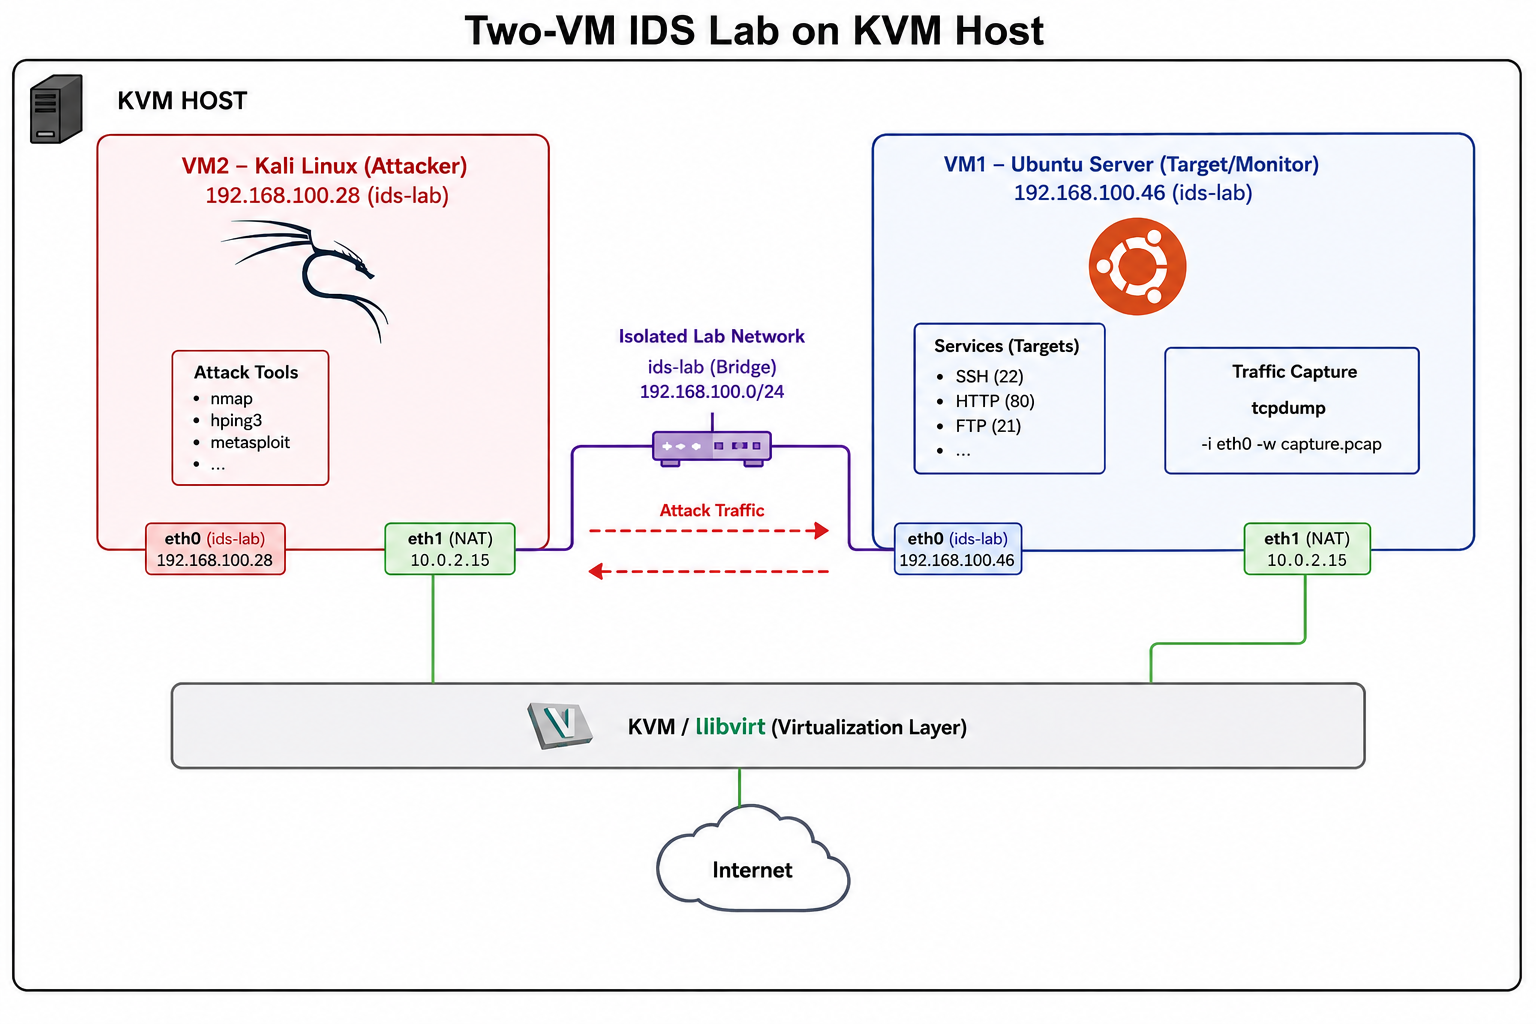
\includegraphics[width=0.74\textwidth]{figures/lab_topology.png}
\caption{Two-machine laboratory on a KVM host. All experimental traffic crosses the isolated \texttt{ids-lab} segment and is captured on the target.}
\label{fig:lab}
\end{figure}

Four captures were recorded, each containing one class of traffic only. Benign traffic consists of repeated HTTP requests to the web server, 21 flows over 22 seconds. An SSH brute force driven by Hydra against port 22 produced 6 flows over 17 seconds. A full nmap SYN scan of all 65,535 ports produced 65,537 flows over 7 seconds. An hping3 SYN flood against port 80 produced 1,523,389 flows over 14 seconds. Because each capture is homogeneous, the tool that generated it labels every flow in it, which is what makes an evaluation of this size possible without manual annotation.

\subsection{Feature Reconciliation}
\label{sec:reconciliation}

Packets are converted to flows with CICFlowMeter, the same tool family that produced the benchmark features. The current release renames many columns relative to the version used for CICIDS-2017, writing \texttt{Dst Port} where the released files write \texttt{Destination Port}, and so on. A mapping restores the training names, the two surviving ratio features are recomputed exactly as in training, and the resulting frame is checked against the frozen 49-feature list stored beside the model. A missing or misnamed column aborts the run rather than silently feeding the model a wrong vector.

% ─────────────────────────────────────────────────────────────
\section{Results}

\subsection{Model Selection}

Table~\ref{tab:models} gives the three candidates on the validation split. The Random Forest leads on every metric, and the margin in F1 comes almost entirely from precision.

\begin{table}[t]
\centering
\caption{Candidate performance on the validation split of 205,653 flows.}
\label{tab:models}
\begin{tabular}{lccccc}
\toprule
\textbf{Model} & \textbf{Precision} & \textbf{Recall} & \textbf{F1} & \textbf{ROC-AUC} & \textbf{PR-AUC} \\
\midrule
Random Forest & \textbf{0.9973} & \textbf{0.9961} & \textbf{0.9967} & \textbf{0.9998} & \textbf{0.9986} \\
CNN           & 0.8713 & 0.9931 & 0.9282 & 0.9986 & 0.9930 \\
LSTM          & 0.8645 & 0.9889 & 0.9225 & 0.9979 & 0.9903 \\
\bottomrule
\end{tabular}
\end{table}

The confusion matrices in Figure~\ref{fig:cmval} show what that difference means operationally. All three models catch nearly every attack, with recall never below 0.988. They are separated by what they do to benign traffic: over the same flows the forest raised 93 false alarms, the CNN raised 4,975 and the LSTM 5,253. Expressed as a precision of 0.87 the gap looks modest; expressed as alerts arriving on an analyst's screen it is more than fifty times the workload for no gain in detection. Since the alert queue is the scarce resource in a real deployment, this is the decisive comparison, and it selects the cheapest and most interpretable of the three candidates.

\begin{figure}[t]
\centering
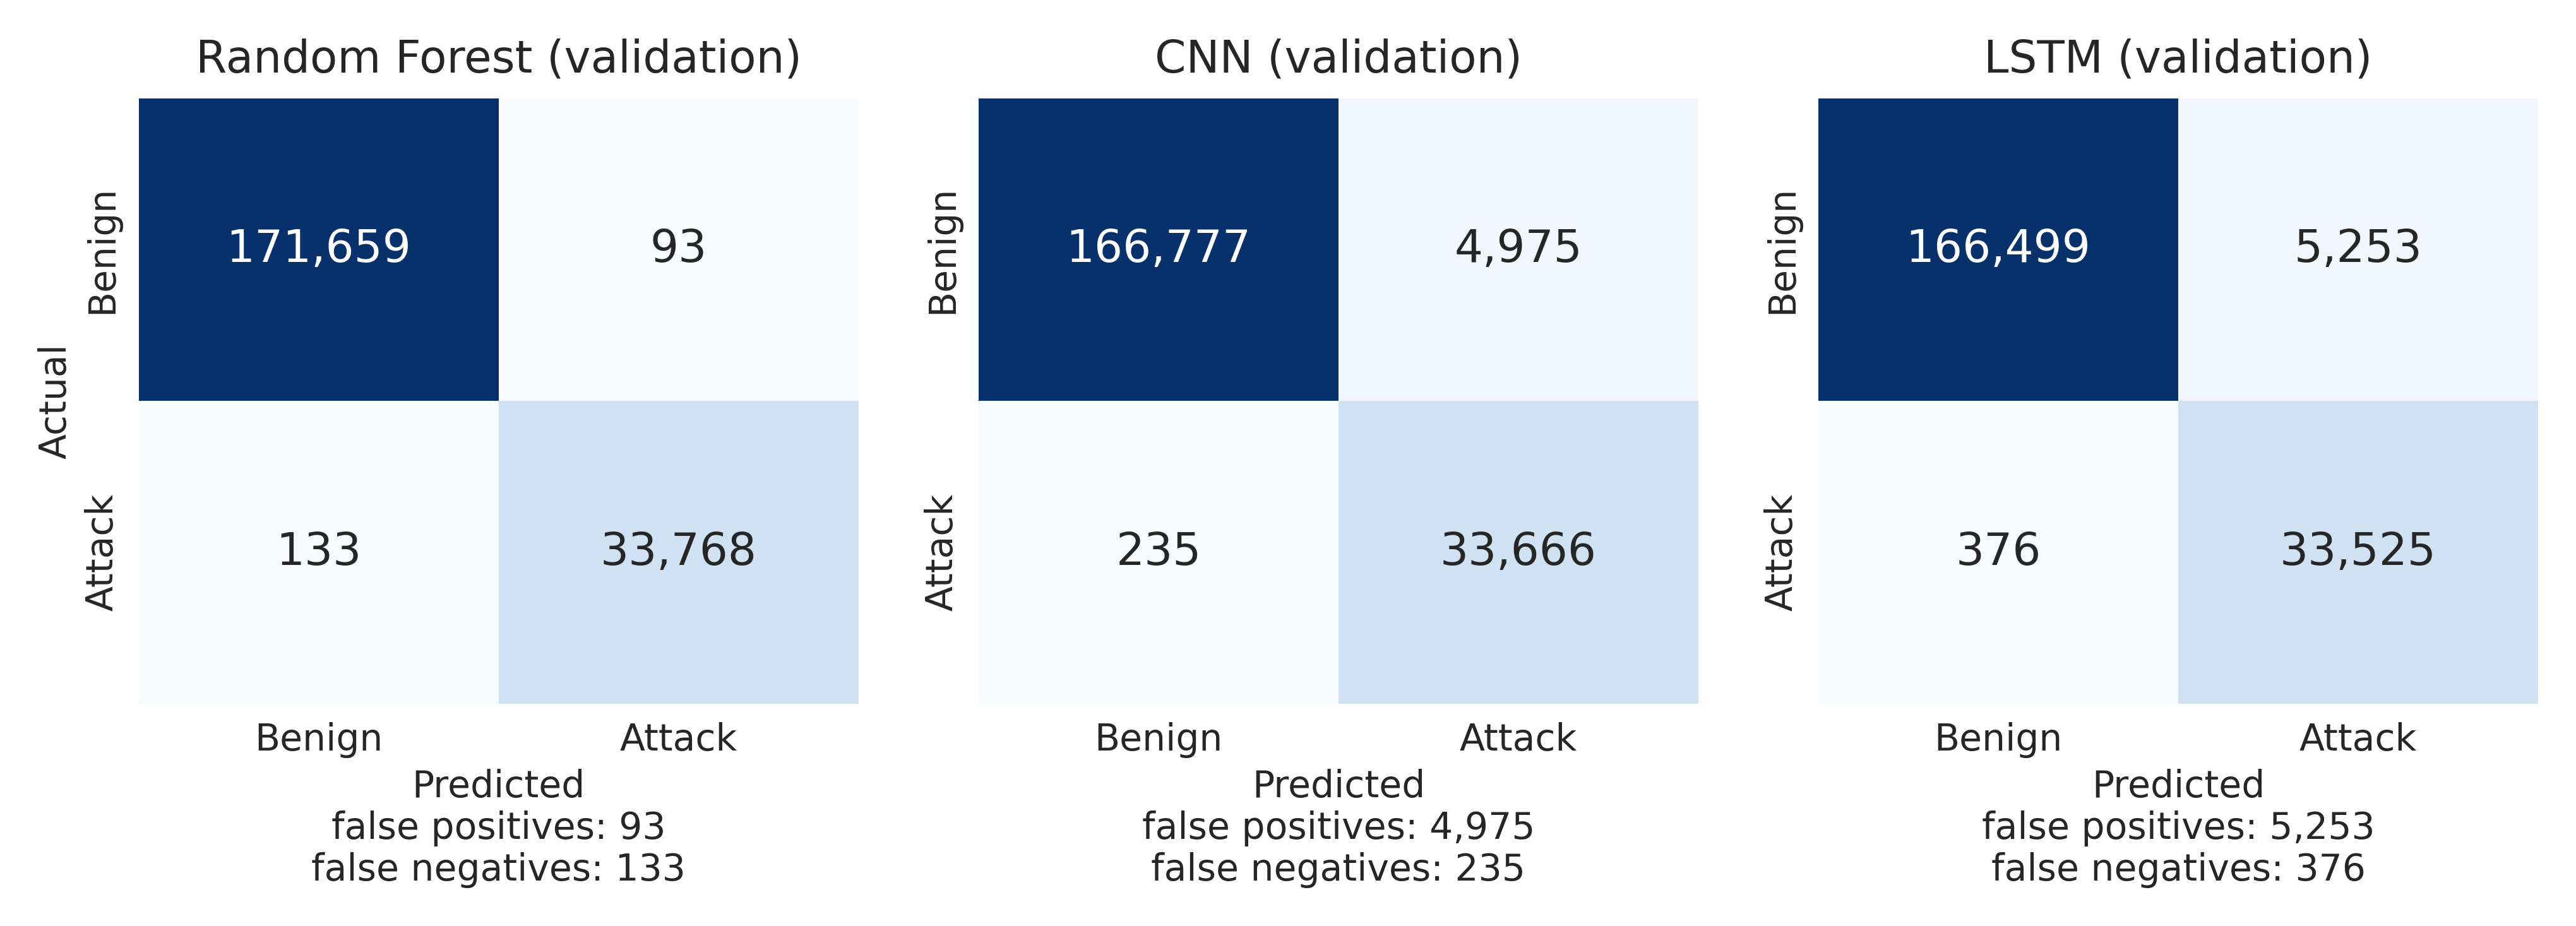
\includegraphics[width=0.94\textwidth]{figures/cm_validation_three_models.png}
\caption{Validation confusion matrices of the three candidates over the same 205,653 flows. The models differ in false positives, not in detection.}
\label{fig:cmval}
\end{figure}

\subsection{Benchmark Performance}

The Random Forest was retrained with 200 trees on the full training set and evaluated once on the held-out test set. Of the 514,132 test flows, 287 benign flows are placed on the attack side and 275 attacks are missed, against 429,380 benign flows and 84,752 attacks. This is a precision of 0.9966, a recall of 0.9968 and an F1 of 0.9967, with a ROC-AUC of 0.9998.

The decision threshold is an operating choice rather than a property of the model. Sweeping it on the validation split and applying the result to the test set moves the detector from a precision of 0.9966 and a recall of 0.9968 at the default 0.5, to a precision of 0.9963 and a recall of 0.9987 at 0.340, which recovers about 160 further attacks for three ten-thousandths of precision. Classification throughput measured on a commodity CPU is 200,000 flows in 4.43 seconds, about 45,000 flows per second, comfortably above the few thousand flows per second our attack scenarios generate.

Extended to the eleven attack types with at least 100 flows, the same model reaches a macro-averaged F1 of 0.92, with nine classes recognised almost perfectly. The two web-attack classes are not: cross-site scripting reaches an F1 of 0.36, with 86 of its 130 flows predicted as web brute force and 60 travelling the other way. At flow level the two are the same object, a short HTTP request to the same server and port, and no feature reveals whether the payload carried a script or a password guess.

\subsection{Explanations}

SHAP attributions were computed with an exact tree explainer over a sample of test flows. The ranking is led by the destination port, the two initial TCP window sizes and the packet-length statistics; one surviving engineered ratio, the forward to backward byte ratio, appears in the top ten. Figure~\ref{fig:beeswarm} adds the direction the ranking hides. Low destination-port values push toward attack and high values toward benign, which reflects that the attacks in this dataset target a small set of service ports while benign clients also talk to many high-numbered ones. Large packet-length variance pushes toward attack, and a large backward initial window pushes toward benign.

\begin{figure}[t]
\centering
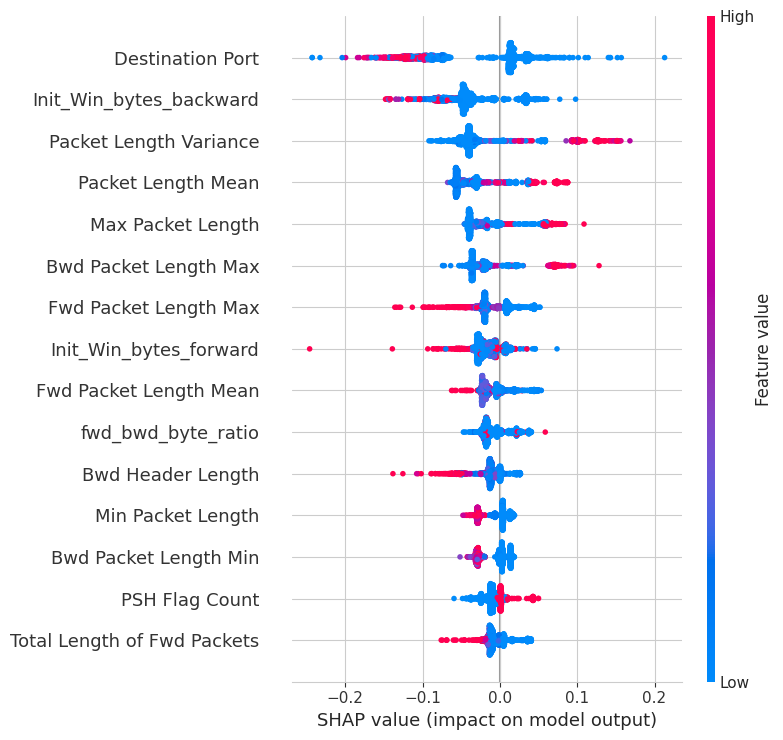
\includegraphics[width=0.62\textwidth]{figures/shap_beeswarm.png}
\caption{SHAP values for individual flows. Each point is one flow, horizontal position is the contribution of that feature to the verdict, and colour is the value of the feature.}
\label{fig:beeswarm}
\end{figure}

The dependence on the destination port is worth stating plainly, because it is the feature least likely to survive a change of network: it encodes which services were attacked during this particular capture campaign rather than what an attack looks like.

\subsection{Evaluation on Independently Generated Traffic}
\label{sec:lab}

The exported model was then run over the four laboratory captures without retraining or tuning. Table~\ref{tab:perattack} reports, for each capture, the number of flows, how many were flagged, and the attack probabilities assigned.

\begin{table}[t]
\centering
\caption{Detection on independently generated laboratory traffic. Every flow is labelled by the tool that produced its capture. The benign row reports false positives, the attack rows report detections.}
\label{tab:perattack}
\begin{tabular}{lrrrrr}
\toprule
\textbf{Traffic type} & \textbf{Flows} & \textbf{Flagged} & \textbf{Rate (\%)} & \textbf{Mean prob.} & \textbf{Max prob.} \\
\midrule
Benign traffic   & 21        & 0 & 0.00  & 0.148 & 0.160 \\
SSH brute force  & 6         & 4 & 66.67 & 0.488 & 0.695 \\
Port scan        & 65,537    & 0 & 0.00  & 0.000 & 0.270 \\
SYN flood (DoS)  & 1,523,389 & 0 & 0.00  & 0.058 & 0.150 \\
\bottomrule
\end{tabular}
\end{table}

Three observations follow. First, the detector produced no false alarm on benign traffic, the behaviour a deployment needs and which the benchmark also predicted. Second, the SSH brute force is the only attack that transfers, and only partially; we treat 66.7\% as directional given a sample of six flows. Third, the two high-volume attacks are missed completely, and not narrowly. The largest attack probability assigned to any of the 1,523,389 flood flows was 0.150, and to any of the 65,537 scan flows 0.270, both below the default threshold of 0.5 and below the tuned operating point of 0.340. Lowering the threshold would not have recovered either attack. The model is not hesitating about this traffic; it is confident that it is benign.

Because every alert carries an explanation, we can ask why the one attack that transfers does so. Figure~\ref{fig:shaplocal} decomposes the highest-scoring brute-force flow. Almost the entire distance from the 0.5 base value to the 0.695 verdict is contributed by a single feature, the destination port being 22, while the packet-shape features of that flow push toward benign. The resemblance that makes this attack transfer is therefore carried mostly by the port, which the training data associates strongly with attacks, and not by the shape of the authentication exchange.

\begin{figure}[t]
\centering
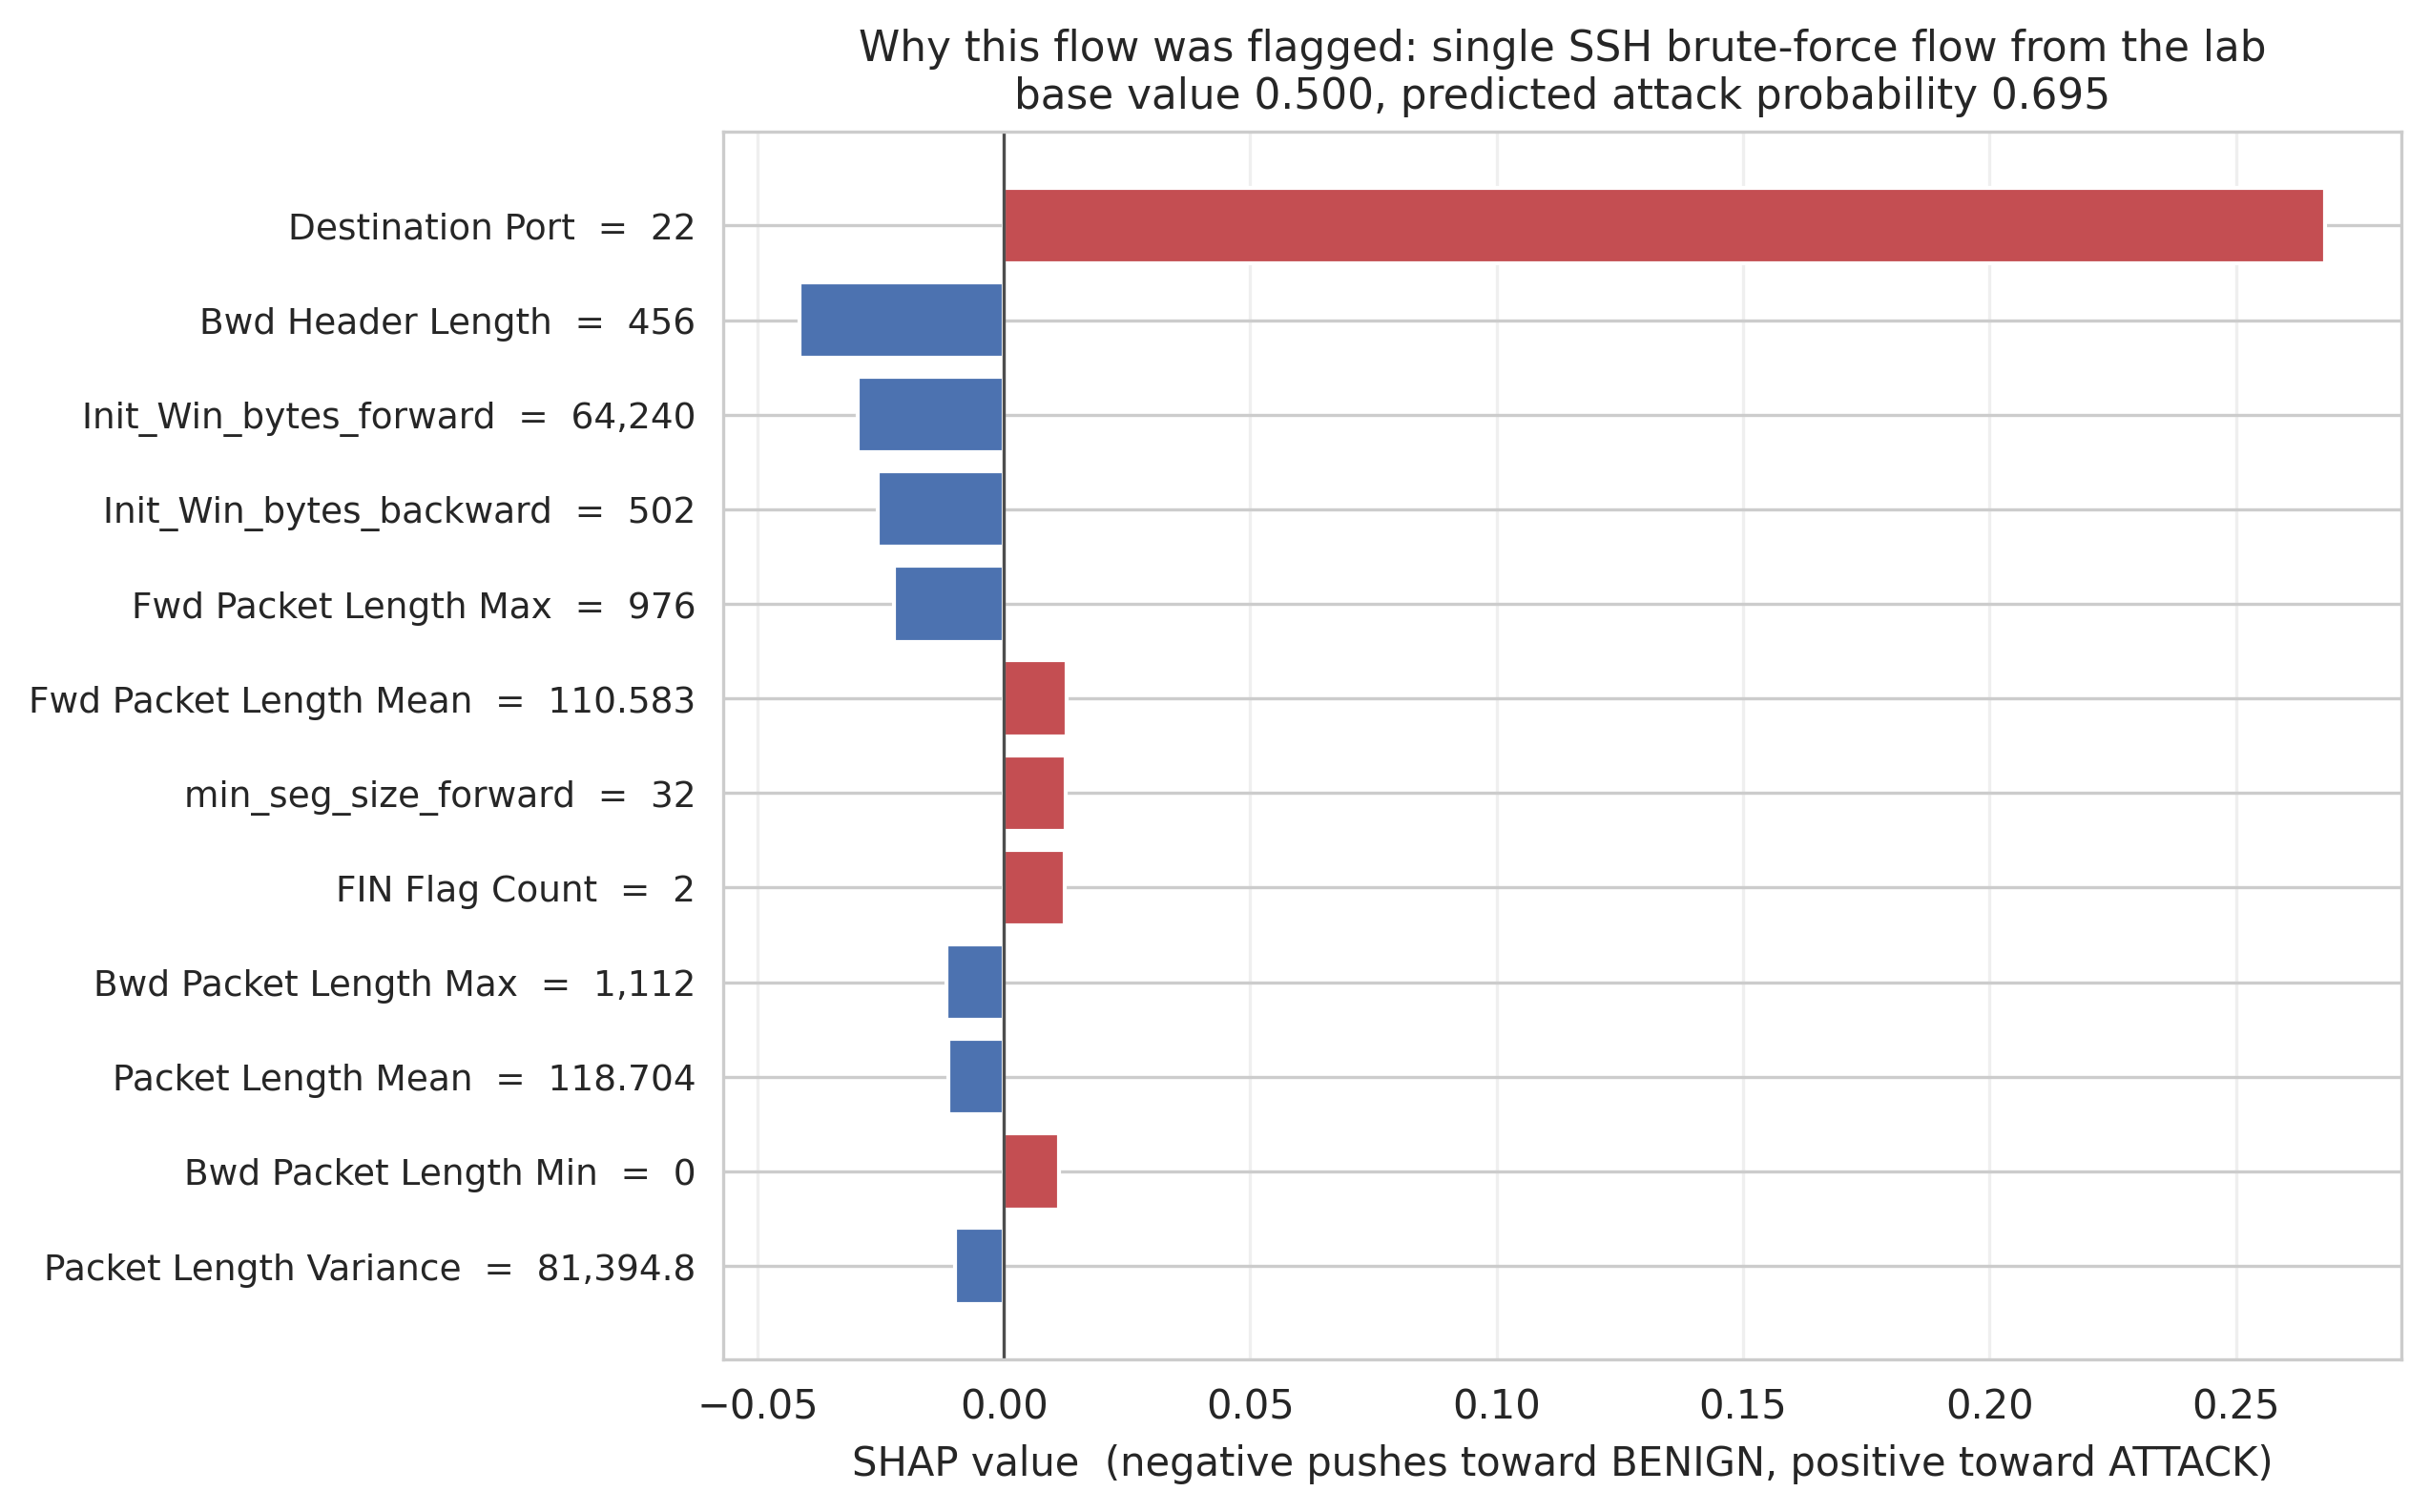
\includegraphics[width=0.74\textwidth]{figures/shap_local_ssh_flow.png}
\caption{Per-alert explanation of one flagged SSH brute-force flow. Red bars push toward attack, blue bars toward benign.}
\label{fig:shaplocal}
\end{figure}

% ─────────────────────────────────────────────────────────────
\section{Discussion}

\subsection{Why the Volumetric Attacks Were Missed}

The failure is not a pipeline defect. The features were renamed, recomputed and validated against the frozen contract before any prediction, and the same pipeline applied to CICIDS-2017 flows reproduces the benchmark behaviour. The cause lies one level down, in what a flow means for each attack.

A SYN flood, as our tool generates it, is a sequence of handshake attempts that carry no data. The modal flow in the capture holds two forward packets and one backward packet, every packet-length statistic is zero, and the median duration is 3.5 milliseconds. What CICIDS-2017 labels DoS and DDoS is a different object: an application-layer HTTP flood of completed connections carrying requests and responses, with a median of four to six forward packets and non-zero payload statistics. A detector that learned the second shape has no reason to react to the first. The two share a name at the level of the label and nothing at the level the model operates on. Figure~\ref{fig:gap} states the contrast.

\begin{figure}[t]
\centering
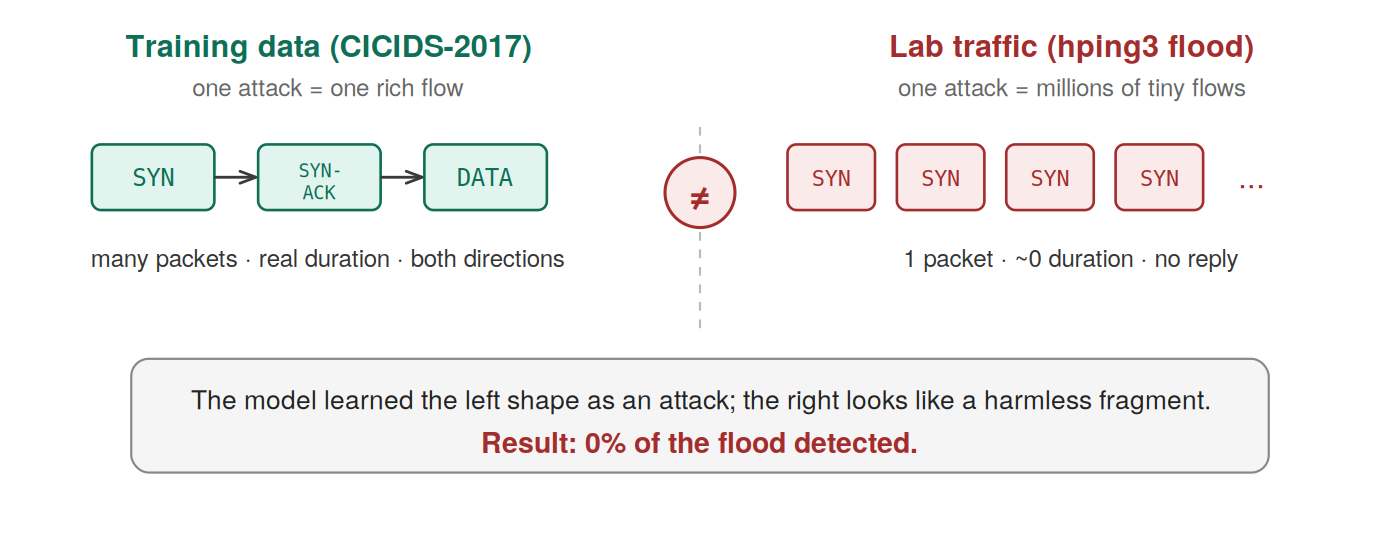
\includegraphics[width=0.76\textwidth]{figures/generalization_gap.png}
\caption{Benchmark attacks and laboratory attacks that share a label but not a flow representation.}
\label{fig:gap}
\end{figure}

The port scan is a harder case and is instructive for that reason. Structurally it resembles the benchmark scan closely: 99.99\% of our scan flows hold one forward and one backward packet, against 99.07\% of the benchmark port-scan flows. Structure alone therefore does not explain this miss, and the remaining difference lies in how individual features are computed on each side of the experiment, which is the subject of the next subsection.

\subsection{Threats to Validity}
\label{sec:limitations}

The most serious threat concerns feature comparability. The released CICIDS-2017 files were produced by a version of CICFlowMeter whose flag counting, packet-length statistics and backward window feature are now documented as defective \cite{engelen2021troubleshooting,rosay2022comprehensive}, while our captures were processed by a later release in which several of these are corrected. Features bearing the same name on both sides are therefore not guaranteed to carry the same meaning, and this confound cannot be separated from the genuine distribution shift without re-extracting both the benchmark packet captures and our own with a single tool version. We regard this as the most important open item, and we note that it is a general hazard for any work that trains on released CICIDS-2017 features and deploys against a current extractor.

Other limitations are narrower. The benign and SSH captures are small, 21 and 6 flows, so those two figures are indicative rather than precise. The laboratory is a two-machine emulation on one hypervisor, not an OpenStack deployment, and covers three attack families. The benchmark evaluation splits flows randomly, which is standard practice but inflates the score relative to a session-wise split. Finally, the detector's reliance on the destination port ties part of the benchmark performance to the service layout of that capture campaign.

\subsection{Towards Hybrid Detection}

The attacks the learned model misses are precisely those other mechanisms detect cheaply. Our flood produced over 1.5 million flows in 14 seconds, roughly 109,000 flows per second from a single address, a figure no legitimate client produces. A rule counting half-open connections per source per second would alarm immediately, at negligible cost, on exactly the traffic the classifier ignores. This argues for a hybrid rather than a better classifier: keep the learned model for what it demonstrably does well, recognising structurally rich multi-packet attacks at a very low false-alarm rate, and pair it with rate-based rules for attacks that announce themselves by volume. The complementarity follows directly from Table~\ref{tab:perattack}.

A second direction is to change the training data rather than the model. Captures produced as in Section~\ref{sec:lab} are labelled by construction and cost no annotation effort, making it practical to extend a benchmark with local traffic and re-extract every feature with one tool version.

% ─────────────────────────────────────────────────────────────
\section{Conclusion}

We trained an intrusion detector on CICIDS-2017 in the conventional way, selected it honestly, and measured it twice. On the benchmark it behaves as the literature predicts: an F1 of 0.9967, a ROC-AUC of 0.9998, about 45,000 flows per second, a false-alarm rate low enough to be operationally usable, and an explanation attached to every decision. On traffic generated a few metres away by real tools it detected none of two high-volume attacks, while correctly leaving benign traffic alone and partially catching a third attack for reasons that turn out to rest largely on a port number.

The contribution is not that benchmark scores can mislead, which has been argued before, but that the gap is here reproduced on our own traces, quantified attack by attack with the decision probability behind each miss, and traced to a concrete cause in the flow representation. A detector scoring 0.997 on a public benchmark cannot be assumed to have learned what an attack is; it has learned what the attacks of that capture campaign looked like after passing through one particular feature extractor.

Three directions follow: the hybrid design above; re-extracting benchmark and laboratory traffic with a single corrected extractor, which would separate the representation shift from the tool artefact; and building training sets from locally generated, self-labelling captures.

\subsubsection{Acknowledgements.}
This work was carried out as an end-of-studies project in the Master programme in Artificial Intelligence and Cybersecurity at the Faculty of Sciences, Ibn Tofail University, Kenitra.

\bibliographystyle{splncs04}
\bibliography{refs}

\end{document}
